% A LaTeX template for MSc Thesis submissions to 
% Politecnico di Milano (PoliMi) - School of Industrial and Information Engineering
%
% S. Bonetti, A. Gruttadauria, G. Mescolini, A. Zingaro
% e-mail: template-tesi-ingind@polimi.it
%
% Last Revision: October 2021
%
% Copyright 2021 Politecnico di Milano, Italy. NC-BY

\documentclass{Configuration_Files/PoliMi3i_thesis}

%------------------------------------------------------------------------------
%	REQUIRED PACKAGES AND  CONFIGURATIONS
%------------------------------------------------------------------------------

% CONFIGURATIONS
\usepackage{parskip} % For paragraph layout
\usepackage{setspace} % For using single or double spacing
\usepackage{emptypage} % To insert empty pages
\usepackage{multicol} % To write in multiple columns (executive summary)
\setlength\columnsep{15pt} % Column separation in executive summary
\setlength\parindent{0pt} % Indentation
\raggedbottom 

% PACKAGES FOR TITLES
\usepackage{titlesec}
% \titlespacing{\section}{left spacing}{before spacing}{after spacing}
\titlespacing{\section}{0pt}{3.3ex}{2ex}
\titlespacing{\subsection}{0pt}{3.3ex}{1.65ex}
\titlespacing{\subsubsection}{0pt}{3.3ex}{1ex}
\usepackage{color}

% PACKAGES FOR LANGUAGE AND FONT
\usepackage[english]{babel} % The document is in English  
\usepackage[utf8]{inputenc} % UTF8 encoding
\usepackage[T1]{fontenc} % Font encoding
\usepackage[11pt]{moresize} % Big fonts

% PACKAGES FOR IMAGES
\usepackage{graphicx}
\usepackage{transparent} % Enables transparent images
\usepackage{eso-pic} % For the background picture on the title page
\usepackage{subfig} % Numbered and caption subfigures using \subfloat.
\usepackage{tikz} % A package for high-quality hand-made figures.
\usetikzlibrary{}
\graphicspath{{./Images/}} % Directory of the images
\usepackage{caption} % Coloured captions
\usepackage{xcolor} % Coloured captions
\usepackage{color}
\usepackage{amsthm,thmtools,xcolor} % Coloured "Theorem"
\usepackage{float}

% STANDARD MATH PACKAGES
\usepackage{amsmath}
\usepackage{amsthm}
\usepackage{amssymb}
\usepackage{amsfonts}
\usepackage{bm}
\usepackage[overload]{empheq} % For braced-style systems of equations.
\usepackage{fix-cm} % To override original LaTeX restrictions on sizes

% PACKAGES FOR TABLES
\usepackage{tabularx}
\usepackage{longtable} % Tables that can span several pages
\usepackage{colortbl}

% PACKAGES FOR ALGORITHMS (PSEUDO-CODE)
\usepackage{algorithm}
\usepackage{algorithmic}

% PACKAGES FOR REFERENCES & BIBLIOGRAPHY
\usepackage[colorlinks=true,linkcolor=black,anchorcolor=black,citecolor=black,filecolor=black,menucolor=black,runcolor=black,urlcolor=black]{hyperref} % Adds clickable links at references
\usepackage{cleveref}
\usepackage[square, numbers, sort&compress]{natbib} % Square brackets, citing references with numbers, citations sorted by appearance in the text and compressed
\bibliographystyle{abbrvnat} % You may use a different style adapted to your field

% OTHER PACKAGES
\usepackage{listings}
\usepackage{pdfpages} % To include a pdf file
\usepackage{afterpage}
\usepackage{lipsum} % DUMMY PACKAGE
\usepackage{fancyhdr} % For the headers
\usepackage{minted}
\fancyhf{}

% Input of configuration file. Do not change config.tex file unless you really know what you are doing. 
% Define blue color typical of polimi
\definecolor{bluepoli}{cmyk}{0.4,0.1,0,0.4}

% Custom theorem environments
\declaretheoremstyle[
  headfont=\color{bluepoli}\normalfont\bfseries,
  bodyfont=\color{black}\normalfont\itshape,
]{colored}

% Set-up caption colors
\captionsetup[figure]{labelfont={color=bluepoli}} % Set colour of the captions
\captionsetup[table]{labelfont={color=bluepoli}} % Set colour of the captions
\captionsetup[algorithm]{labelfont={color=bluepoli}} % Set colour of the captions

\theoremstyle{colored}
\newtheorem{theorem}{Theorem}[chapter]
\newtheorem{proposition}{Proposition}[chapter]

% Enhances the features of the standard "table" and "tabular" environments.
\newcommand\T{\rule{0pt}{2.6ex}}
\newcommand\B{\rule[-1.2ex]{0pt}{0pt}}

% Pseudo-code algorithm descriptions.
\newcounter{algsubstate}
\renewcommand{\thealgsubstate}{\alph{algsubstate}}
\newenvironment{algsubstates}
  {\setcounter{algsubstate}{0}%
   \renewcommand{\STATE}{%
     \stepcounter{algsubstate}%
     \Statex {\small\thealgsubstate:}\space}}
  {}

% New font size
\newcommand\numfontsize{\@setfontsize\Huge{200}{60}}

% Title format: chapter
\titleformat{\chapter}[hang]{
\fontsize{50}{20}\selectfont\bfseries\filright}{\textcolor{bluepoli} \thechapter\hsp\hspace{2mm}\textcolor{bluepoli}{|   }\hsp}{0pt}{\huge\bfseries \textcolor{bluepoli}
}

% Title format: section
\titleformat{\section}
{\color{bluepoli}\normalfont\Large\bfseries}
{\color{bluepoli}\thesection.}{1em}{}

% Title format: subsection
\titleformat{\subsection}
{\color{bluepoli}\normalfont\large\bfseries}
{\color{bluepoli}\thesubsection.}{1em}{}

% Title format: subsubsection
\titleformat{\subsubsection}
{\color{bluepoli}\normalfont\large\bfseries}
{\color{bluepoli}\thesubsubsection.}{1em}{}

% Shortening for setting no horizontal-spacing
\newcommand{\hsp}{\hspace{0pt}}

\makeatletter
% Renewcommand: cleardoublepage including the background pic
\renewcommand*\cleardoublepage{%
  \clearpage\if@twoside\ifodd\c@page\else
  \null
  \AddToShipoutPicture*{\BackgroundPic}
  \thispagestyle{empty}%
  \newpage
  \if@twocolumn\hbox{}\newpage\fi\fi\fi}
\makeatother

%For correctly numbering algorithms
\numberwithin{algorithm}{chapter}
\usepackage{listings}
\usepackage{xcolor}

\definecolor{mediumgray}{rgb}{0.3, 0.4, 0.4}
\definecolor{mediumblue}{rgb}{0.0, 0.0, 0.8}
\definecolor{forestgreen}{rgb}{0.13, 0.55, 0.13}
\definecolor{darkviolet}{rgb}{0.58, 0.0, 0.83}
\definecolor{royalblue}{rgb}{0.25, 0.41, 0.88}
\definecolor{crimson}{rgb}{0.86, 0.8, 0.24}

\lstdefinelanguage{JavaScript}{
  morekeywords=[1]{break, continue, delete, else, for, function, if, in,
    new, return, this, typeof, var, void, while, with},
  % Literals, primitive types, and reference types.
  morekeywords=[2]{false, null, true, boolean, number, undefined,
    Array, Boolean, Date, Math, Number, String, Object},
  % Built-ins.
  morekeywords=[3]{eval, parseInt, parseFloat, escape, unescape},
  sensitive,
  morecomment=[s]{/*}{*/},
  morecomment=[l]//,
  morecomment=[s]{/**}{*/}, % JavaDoc style comments
  morestring=[b]',
  morestring=[b]"
}[keywords, comments, strings]

\lstdefinestyle{JSES6Base}{
  backgroundcolor=\color{white},
  basicstyle=\ttfamily,
  breakatwhitespace=false,
  breaklines=false,
  captionpos=b,
  columns=fullflexible,
  commentstyle=\color{mediumgray}\upshape,
  emph={},
  emphstyle=\color{crimson},
  extendedchars=true,  % requires inputenc
  fontadjust=true,
  frame=single,
  identifierstyle=\color{black},
  keepspaces=true,
  keywordstyle=\color{mediumblue},
  keywordstyle={[2]\color{darkviolet}},
  keywordstyle={[3]\color{royalblue}},
  numbers=left,
  % numbersep=5pt,
  numberstyle=\tiny\color{black},
  rulecolor=\color{black},
  showlines=true,
  showspaces=false,
  showstringspaces=false,
  showtabs=false,
  stringstyle=\color{forestgreen},
  tabsize=2,
  title=\lstname,
  upquote=true  % requires textcomp
}

\lstdefinestyle{JavaScript}{
  language=JavaScript,
  style=JSES6Base
}
\lstdefinestyle{ES6}{
  language=ES6,
  style=JSES6Base
}


%----------------------------------------------------------------------------
%	NEW COMMANDS DEFINED
%----------------------------------------------------------------------------

% EXAMPLES OF NEW COMMANDS
\newcommand{\bea}{\begin{eqnarray}} % Shortcut for equation arrays
\newcommand{\eea}{\end{eqnarray}}
\newcommand{\e}[1]{\times 10^{#1}}  % Powers of 10 notation

%----------------------------------------------------------------------------
%	ADD YOUR PACKAGES (be careful of package interaction)
%----------------------------------------------------------------------------

%----------------------------------------------------------------------------
%	ADD YOUR DEFINITIONS AND COMMANDS (be careful of existing commands)
%----------------------------------------------------------------------------

%----------------------------------------------------------------------------
%	BEGIN OF YOUR DOCUMENT
%----------------------------------------------------------------------------
\begin{document}

\fancypagestyle{plain}{%
\fancyhf{} % Clear all header and footer fields
\fancyhead[RO,RE]{\thepage} %RO=right odd, RE=right even
\renewcommand{\headrulewidth}{0pt}
\renewcommand{\footrulewidth}{0pt}}

%----------------------------------------------------------------------------
%	TITLE PAGE
%----------------------------------------------------------------------------

\pagestyle{empty} % No page numbers
\frontmatter % Use roman page numbering style (i, ii, iii, iv...) for the preamble pages

\puttitle{
	title=Data Information Quality Project,
    subtitle= Completeness and Distinctness Quality Issues Analyses on a Regression Problem,
	name1=Irfan Cela - 10694934,
	name2=Bianca C. Savoiu Marinas - 10684465,
	academicyear=2023-2024,
	groupnumber=27
} % These info will be put into your Title page 

%----------------------------------------------------------------------------
%	PREAMBLE PAGES: ABSTRACT (inglese e italiano), EXECUTIVE SUMMARY
%----------------------------------------------------------------------------
\startpreamble
\setcounter{page}{1} % Set page counter to 1

%----------------------------------------------------------------------------
%	LIST OF CONTENTS/FIGURES/TABLES/SYMBOLS
%----------------------------------------------------------------------------

% TABLE OF CONTENTS
\thispagestyle{empty}
\tableofcontents % Table of contents 
\thispagestyle{empty}
\cleardoublepage

%-------------------------------------------------------------------------
%	THESIS MAIN TEXT
%-------------------------------------------------------------------------
% In the main text of your thesis you can write the chapters in two different ways:
%
%(1) As presented in this template you can write:
%    \chapter{Title of the chapter}
%    *body of the chapter*
%
%(2) You can write your chapter in a separated .tex file and then include it in the main file with the following command:
%    \chapter{Title of the chapter}
%    \input{chapter_file.tex}
%
% Especially for long thesis, we recommend you the second option.

\addtocontents{toc}{\vspace{2em}} % Add a gap in the Contents, for aesthetics
\mainmatter % Begin numeric (1,2,3...) page numbering

\definecolor{codegreen}{rgb}{0,0.6,0}
\definecolor{codegray}{rgb}{0.5,0.5,0.5}
\definecolor{codepurple}{rgb}{0.58,0,0.82}
\definecolor{backcolour}{rgb}{0.95,0.95,0.92}

\lstdefinestyle{mystyle}{
    backgroundcolor=\color{backcolour},   
    commentstyle=\color{codegreen},
    keywordstyle=\color{magenta},
    numberstyle=\tiny\color{codegray},
    stringstyle=\color{codepurple},
    basicstyle=\ttfamily\footnotesize,
    breakatwhitespace=false,         
    breaklines=true,                 
    captionpos=b,                    
    keepspaces=true,                 
    numbers=left,                    
    numbersep=5pt,                  
    showspaces=false,                
    showstringspaces=false,
    showtabs=false,                  
    tabsize=2
}
\lstset{language=SQL, style=mystyle}


\chapter{Assigned Data quality issues and Machine Learning task}
\label{ch:chapter_1}%
% The \label{...}% enables to remove the small indentation that is generated, always leave the % symbol.

\section{Problem description}
\label{sec:section_1_1}%
In this problem, we are tasked with investigating data quality issues, specifically focusing on completeness and distinctness, within a regression problem. The dataset is initially generated using the \verb|make_dataset_regression()| function from the \verb|scikit-learn| library. Subsequently, errors related to completeness and distinctness are intentionally introduced, creating pollution within the dataset. The primary objective is to address these issues and then evaluate their impact on the regression problem.

\chapter{Setup choices}
\label{ch:chapter_2}%

\section{Completeness}
\label{sec:section_2_1}%
In the context of data completeness in a regression problem, completeness refers to the extent to which the dataset is free from missing values. Missing values can significantly impact the performance and reliability of regression models, so it's crucial to explore different scenarios and distributions of missing values. 

\subsection{Data collection phase}
\label{subsec:section_2_1_1}%
The data was not collected from external sources or loaded from a file, because the problem uses some artificial created dataset. To create the dataset we use the \verb|sklearn| function \verb|make_dataset_for_regression| creating 1000 or more samples, in some experiments an increasing number of samples, until 2000 data points. We start with a set in which we consider 3 features and all of them informative, a target, and we have no noise and no bias in the creation of the data and we select a random seed in order to have reproducible data.

\subsection{Experiments on completeness}
\label{subsec:section_2_1_2}%
The experiments we decided to perform are the following:
\begin{enumerate}
\item[0.] \textbf{Baseline with complete data}: We decided to consider also a baseline with complete data in order to see how much the pollution experiments worsen the behavior of the models, understanding their changes also in comparison with a ideal state. 
\item[1.] \textbf{Low percentage of values MCAR and different imputations}: In this experiment with a pollution function we generate a random mask randomly, in order to create some missing incompleteness in the DataFrame, of a chosen maximum percentage value. In this case we want to analyze the behavior of the models in case of a low percentage of MCAR, so in the experiment we use a percentage range that goes from 0.025 to 0.25 with a step of 0.025. Without any data imputation we got some expected results, that represent the fact that with the increasing percentage of MCAR values the performance on the train test gets worse, having an increase of the RMSE, especially in the GPRegressor, that behaves worst than the other algorithms. We can also see that this last model is the one that also overfits the most, while the others are pretty much stable, having some increasing behavior, but of a small range, in the KNNRegressor. Trying different imputations we observed that:
\begin{enumerate}
    \item Imputing the median: the behavior remains the same as in case of no imputation, but the no imputation case is actually a constant imputation of '0', because otherwise the algorithms wouldn't work, not accepting null values; so we can say that the imputation of the median behaves almost as the imputation of the constant value '0', with really small improvements in some error growth, but not an important one
    \item Imputing the mean: the behavior is almost the same in all the models, with little, non important changes
    \item Imputing the most frequent value: we have some different behaviors for the models, but in general this kind of imputation seems to worsen the behavior of all algorithms, comparing it with the imputation of the constant value '0'
    \item Imputing the standard deviation: this type of imputation performs really good with the GPRegressor with respect to the previous cases, but it worsens the RMSE growth in all the other experiments, having a bigger error since the lowest MCAR values until the last percentage. It improves the GPRegressor not only regarding the train performance, but also reducing a lot the overfitting, having a better prediction 
    \item Imputing with the KNN or the Linear Regressor: the behavior is the same as in case of imputing the standard deviation, with really small differences in the trends, nothing relevant that could distinguish this imputation for the others
\end{enumerate}
Seeing the behaviors with the different imputations techniques, we can conclude that they don't give big results in this case, having an artificial dataset with 3 features, all of them important. Given the fact that we didn't see important improvements with more complex imputations we will use in the following experiments always the median imputation, in order to see how it behaves in different conditions, changing also the feature's importance and the degree of incompleteness. 
\item[2.] \textbf{High percentage of values MCAR}: Exactly like before we performed some experiments on MCAR, with different percentages, trying in this case to analyse more incomplete data with a range that goes from 0.275 to 0.50, maintaining the same setting of three features and all of them considered informative ones. As before in the models we can see an increase in the RMSE in correspondence of the increasing percentage of missing values, but in this case we have a different behavior for the GPRegressor, that instead with a high percentage of MCAR values starts to decrease its RMSE, but nonetheless its performance in the training remains the worst, having a big magnitude difference with the other ones; and also in the distance between train and test performance this is the model that performs worst. The others remain pretty much stable looking at the regression distance train-test. After imputing the median to clean the data in this case the GPRegressor has a even worse behavior in the performance while the others remain almost the same.
\item[3.] \textbf{Fixed MCAR for different features in the dataset}: In this case we increased the number of features present in the dataset in order to have a broader experiment on the MCAR for different features. So we chose to create a dataset with 10 features, from which only 5 are considered informative, in order to explore different behaviors and see how much this could impact the model. In general the RMSE and the distance between train and test is stable, so it doesn't change so much from a feature to the other. We have some features that seem to affect more the behavior of the algorithms, and
seeing some different behaviors in the results we can imagine that the different importance of the feature influenced the algorithm and this is why we decided to make further analyses on important and not important features in some of the next experiments. Also in this case in the cleaning phase the median doesn't change much the behavior, unfortunately it seems to worsen some behaviors, again the one of the GPRegressor.
\item[4.] \textbf{Different percentages of values MCAR for each feature in an increasing dataset}: in this experiment polluting with MCAR values for each feature in an incremental way, also in an incrementing dataset, we see some strange behaviors, that cannot be smoother by the imputation of the median, and we can't retrieve much information from these patterns, so we conclude that there are too many variables and randomness in this experiment, so we have to make more precise and focused experiments, varying only some aspects each time. Also we can imagine that the increasing data try to balance the increasing MCAR, having opposing components that create the erratic trend.
\item[5.] \textbf{MAR in an increasing dataset}: As in the MCAR experiment we generate a random mask, now for incompleteness (MAR) and introduce NaN values in the DataFrame according to the generated mask. We introduce missing values in a way that depends on the values of other specific features and simulate a non-random incompleteness pattern based on the values of certain features. In this case based on the \verb|feature_referenced| and \verb|feature_dependent| chosen, the features 1 and 2, if the \verb|feature_referenced| has some values above 100, in the correspondent element in the \verb|feature_dependent| we put a NaN value, creating a MAR incompleteness. As before from the results we see an oscillating behavior, so we can say that the MAR influences negatively the model, but the increasing of samples in the dataset tries to balance this effect, and limiting in some sense the RMSE. In this case we can notice that the Linear Regressor and the Bayesian Ridge are almost not influenced by the null values in the dataset, having the best behavior, with a RMSE almost equal to zero and no different between training and testing, not overfitting the dataset; but also in this case the imputation of the median doesn't help much the algorithms to improve their behavior.
\item[6.] \textbf{MNAR in an increasing dataset}: In this case we generate a random mask for incompleteness (MNAR) and introduce NaN values in the DataFrame according to the generated mask. We introduce missing values in a way that depends on the values of specific features and simulate a non-random incompleteness pattern based on the values of certain features. We create a constraint for a column, so if the feature has a certain range (i.e. in this case a range between 51 and 149) of values we make the value NaN, creating in this way a non-random incompleteness pattern, depending on the value of the feature itself. The results of this experiment are almost the same as the one before, so the kind on missing value MNAR or MAR doesn't influence the model, because the values are artificially created and don't have particular meaning for these rules to have a certain impact.
\item[7.] \textbf{Different percentages of values MCAR for the most informative features}: In this experiment we focus on the most important features of the dataset, so we first split the data in training and testing in order to train and apply a Random Forest Regressor model. From the Random Forest we then extract the rank of the most important features and for this experiment consider the most important features only the first 3 in the ranking, that will be polluted with different percentages from 0.05 to 0.50 of incomplete values. For this experiment in order to have more feature and relevant features we extended the dataset, having 9 features with 4 informative ones. From the results we can see that increasing the percentage of MCAR values in the most important features of the model we get a linear increase of the RMSE, while the models don't overfit too much, having a similar behavior between training and testing, with an increasing error mainly for the GPRegressor, as in all experiments done so far. We can see that the important features, as expected, have a relevant impact on our algorithms and the missing values are a critical problem, that cannot be solved by simply imputing the median value instead of the NaN, because we still lose useful information for the problem. 
\item[8.] \textbf{Different percentages of values MCAR for the less informative features}: As for the precedent experiment, in this one, in order to extract the less informative features, we used the same procedure, training a Random Forest Regressor model and extracting the ranking of the features, but this time selecting the last three features of the ranking. We also use the same percentages of incomplete MCAR values seen in the previous experiment, but in this case we can see that the influence is really small, so all the algorithms keep their behavior stable, even if increasing a lot the percentage of missing values, and this is because being less informative features they don't impact so much the model. The already stable behavior is kept also stable imputing the median, without relevant results.
\item[9.] \textbf{Different percentages of values MNAR mixing informative and non informative values}: Mixing the two experiments performed before, keeping the same range of percentages for missing values, but performing both a pollution on the most informative and less informative features we get almost the same result as for the experiment of the most informative features. In almost all the models we find again the increasing linear error with the increasing of the percentage of incompleteness and in this cases the behavior is similar to the experiment 7, so we can imagine that the most informative features influence the most the model, while the less informative ones have a little impact. We can see an interesting behavior in the GPRegressor, though, in which combining the two pollution methods we have an exponential increase in the RMSE and the difference between train and test results, having that the combination of important and less important features create an exponential problem when dealing with incompleteness, that cannot be solved by imputing the median. 
\item[10.] \textbf{Different percentages combination of values MCAR and MNAR}: In the last experiment on completeness we decided to mix together different percentages of MCAR from 0.05 to 0.5 and some changing MNAR features on ten different datasets. We discover again an incremental behavior of the RMSE, with an abrupt increase in the GPRegressor after a certain threshold of missing values, while the other maintain a linear increasing behavior, and an almost stable trend in the difference between training and testing. 
\end{enumerate}
In all the previous experiments we didn't see particular changes in the time needed to run the models, so we never commented the speed because this doesn't influence much our analysis. In general we can assess that the MLP Regressor, being a more sophisticated and complex Regressor takes a longer time to be executed, and also GPRegressor can require more time than the others, but among the different experiments the changes were small, sometimes of around a few seconds. 

\section{Distinctness}
\label{sec:section_2_2}%

\subsection{Data collection phase}
\label{subsec:section_2_2_1}%

\subsection{Experiments on distinctness}
\label{subsec:section_2_2_2}%
The experiments we decided to perform are the following:
\begin{enumerate}
\item[1.] \textbf{Mid-high distinctness in a random feature}
For the first experiment, we selected a random column from the artificial dataset and focused on its pollution. Then, we randomly selected a value from the column and pasted it into another cell. We repeated this process until the distinctness index of the column was reduced to the target percentage or lower. We tested the dataset for non-distinctness percentages ranging from 0\% to 50\%.

The results indicate that the GP Regressor model performs poorly because it is unable to construct a probability model based on the unchanged target, resulting in worse performance than in the cleaned dataset. Overall, regardless of the percentage of non-distinct values, the other models performed worse than expected. However, they all had similar performances on the test set, with the distances between the train and test performances being close to zero for all models except for GP Regressor and KNN Regressor, which had slightly better performances over the train set. In the speed plots, nothing remarkable is noticeable since the MLP Regressor always trains slower than others, and the GP Regressor takes more time than simpler models like the Linear Regressor.

\item[2.] \textbf{Low distinctness inside an informative column}
In the second experiment, we continued the first one but with higher percentages of non-distinct values (i.e., lower percentages of distinctness, ranging from 50\% to 100\%). The performances improved as the distinctness decreased because the models approximated the features with a single value, discarding the information of that feature and focusing on the others. However, the error saturates to a single value since the models have lost a component of the search space. As a result, they will never achieve high performance.

\item[3.] \textbf{Fixed Distinctness of Different Datasets}
For the third experiment, we fixed the distinctness percentage at 80\% and trained the models on datasets with increasing samples. Also in this case we have applied the pollution function used in the previous two experiments, so the experiments pollutes just one feature over the entire dataset.

 In this case, it is observed that the performance is poor and is dependent on the number of samples chosen. The performance graph fluctuates with each iteration, making it difficult to determine the cause. This indicates that the distinctness of a single column has a significant impact on the final model. The experiment affects velocities, as demonstrated by the MLP Regressor. Reducing the uniqueness index within a feature leads to longer training times.

\item[4.] \textbf{Different Percentages among Features}
In the fourth experiment, we decided to modify the dataset creation function by increasing the number of features to nine and the number of informative features to four. This is because we wanted to see if the general change of most features would cause a drop in model performance or if there would be no changes. The distinctness percentages imposed on the selected features are similar, although not identical, in order to avoid changing all columns in the same way.

The results showed that all models performed poorly overall, regardless of any changes made. Additionally, only the GP Regressor performed better in the training set compared to the test set. The speed plot did not reveal any unexpected results.

\item[5.] \textbf{Random Noise}
For the fifth experiment, we introduced general noise throughout the dataset to test the models' sensitivity to approximate data. Specifically, we varied the noise's variance (from 0.00625 to 0.0625) at each iteration.

Despite a small change in the data, model performance worsened. However, performance remained similar in the two model evaluation sets. It is important to note that the performance of the previously best-performing models worsens linearly with increasing noise, highlighting the significance of data filtering in achieving a good model.

\item[6.] \textbf{Categorical Variables}
For the sixth experiment, we discretized the values of a random feature. We increased the number of ranges generated for data approximation by one unit at each iteration.

The results are quite surprising. Although previous experiments have shown how distinctness is an important element that can compromise the reliability of the chosen model, in this case, we note that discretization has a beneficial effect on both the training and test sets. With larger ranges, the performance deviates from the baseline. However, as the number of ranges increases up to 10, the performance of all models improves significantly. The only exception to this is the GP Regressor, which performs worse than the previous cases.

\item[7.] \textbf{Outliers}
In the seventh experiment, we randomly modified some of the data to create outliers within the dataset.  To do this, we randomly extracted rows and columns (separately) to be selected for modification, and assigned them a random value between 0 and 100. In this way, a few values would have been seen as correct, while those with a very large value would have been visibly outliers.

The performance of all models has significantly worsened, as has the distance between the performance of the training and testing phases. The KNN Regressor is the only model capable of addressing this problem, as it searches for the closest samples to process the outcome. This way, KNN is able to handle the problem of outliers, while simple models like Linear Regressor are no longer good models.

\item[8.] \textbf{High and Low Distinctness Combined}
The eighth experiment is similar to the fourth experiment, but this time we only modified two random features of the dataset in opposite ways. In particular, we modified the first one by reducing the distinctness to meet the chosen criteria, while in the second case, we kept it high, albeit slightly lower than the original.

Despite the similarity to the aforementioned experiment, the results are significantly different. In fact, the performance of all models worsens by approximately 10 times, clearly demonstrating how the alteration of two features inhibits the models from extracting the necessary information for predicting the target. However, the difference between the performance of the training and testing phases is very similar, as in experiment four. There is nothing evidently important regarding the execution times.

\item[9.] \textbf{Distinctness over Most Informative Feature}
For our ninth experiment, we chose to increase the number of features available in the dataset to nine and the informative features to four. This is because we wanted to modify the most informative feature (found in the same way as it was done in some completeness experiments), in order to notice if changes to the original distinctness cause problems in the final models.

The results indicate a general decline in the performance of all models. However, it is noteworthy that the GP Regressor did not perform worse, as it did in all previous experiments. However, all models demonstrate a strong influence, as expected, from the information contained in the selected feature.
\item[10.] \textbf{Distinctness over Less Informative Feature}
In the last experiment, as in the ninth, we generated a dataset with nine features, four of which are informative. In this case, we explored the dependencies of the models with the least important features (according to the evaluation system used in the previous experiments).

The results are surprising in some respects when compared to the baseline. The models' performance worsens even if they are distinct, settling around high values. Modifying the values contained in the non-informative feature would therefore be... Modifying the values contained in the non-informative feature is crucial, even if they are considered unimportant.
\end{enumerate}


\chapter{Pipeline implementation}
\label{ch:chapter_3}%

\section{Completeness}
\label{sec:section_3_1}%

\subsection{Pipeline description}
\label{subsec:section_3_1_1}%

In the completeness experiments after creating the dataset, we polluted it with different functions, changing the percentage of the completeness, the size of the dataset and the kind of completeness. After applying the specific pollution function we analyze the results of the regression models, that were executed after performing an imputation of a constant value '0', otherwise the models do not work with null values. 
After this analysis, in the pipeline we add the data preparation phase, and after trying different data imputation techniques without any remarkable results we decided to use the imputation of the median value and see if it improves the behavior of the models in the different experiments. After the data preparation phase we plot again the results of the algorithms on the cleaned data and confront them with the previous ones. Comparing the plots we never see important changes after the data preparation.


\section{Distinctness}
\label{sec:section_3_2}%

\subsection{Pipeline description}
\label{subsec:section_3_2_1}%

In the distinctness experiments differently from completeness we do not have the data preparation phase, we only create the dataset and then pollute it, also with different percentages of distinctness, with different sizes of the dataset and different kinds of distinctness, like using outliers and random noise to analyze the algorithms behavior. After polluting the dataset we perform the training and the testing with each one of the Regression models chosen for the analysis and we plot the results, analyzing how much the distinctness impacts on our models, given also different settings of the dataset.

%*******************************************************************************************************
\chapter{Results}
\label{ch:chapter_4}%

\section{Completeness}
\label{sec:section_4_1}%

\subsection{Main results of the completeness experiments}
\label{subsec:section_4_1_1}%
Based on the experiments conducted on the completeness in a regression problem, we draw the following conclusions:
\begin{enumerate}
    \item Impact of Incompleteness on Model Performance:
        Introduction of incompleteness generally leads to worse model performance, especially when null values are present in the most informative features. This suggests that missing data in crucial variables can significantly hinder the model's ability to make accurate predictions.
    \item Limited Effectiveness of Imputations:
        Imputations were found to be insufficient in addressing data quality problems. While they enabled the ML algorithms to run, they did not effectively resolve the underlying issues, resulting in a persistent increase in error. This indicates that imputations alone may not be a robust solution for handling missing data in regression problems.
    \item Limited Effectiveness of Imputations:
        Imputations were found to be insufficient in addressing data quality problems. While they enabled the ML algorithms to run, they did not effectively resolve the underlying issues, resulting in a persistent increase in error. This indicates that imputations alone may not be a robust solution for handling missing data in regression problems.
    \item Absence of Pronounced Overfitting:
        Despite the increase in error during training due to incompleteness, there wasn't a noticeable occurrence of overfitting. The difference between training and testing results remained stable. This suggests that the models were not excessively adapting to the noise introduced by incomplete data, and their generalization to unseen data was consistent.
    \item GPRegressor's Poor Performance:
        The GPRegressor exhibited the worst performance among the tested algorithms. Its behavior was particularly erratic and showed significant variability across different experiments. This suggests that Gaussian Process regression may be more sensitive to the presence of missing data compared to other regression algorithms.
    \item Almost no impact on speed:
        The consistent speed of algorithm execution across different experiments is an additional noteworthy conclusion. This finding suggests that, despite variations in data completeness and the associated challenges, the computational efficiency of the algorithms remained relatively stable. The consistent speed implies that the time required to perform each algorithm is not significantly influenced by the presence of incomplete data. This stability in execution time is anyway a valuable information, as it indicates that the algorithms try to handle missing data without causing notable delays.
\end{enumerate}
To confirm our conclusions we show some of the most important graphs for completeness.

\newpage
\begin{figure}[H]
    \centering
    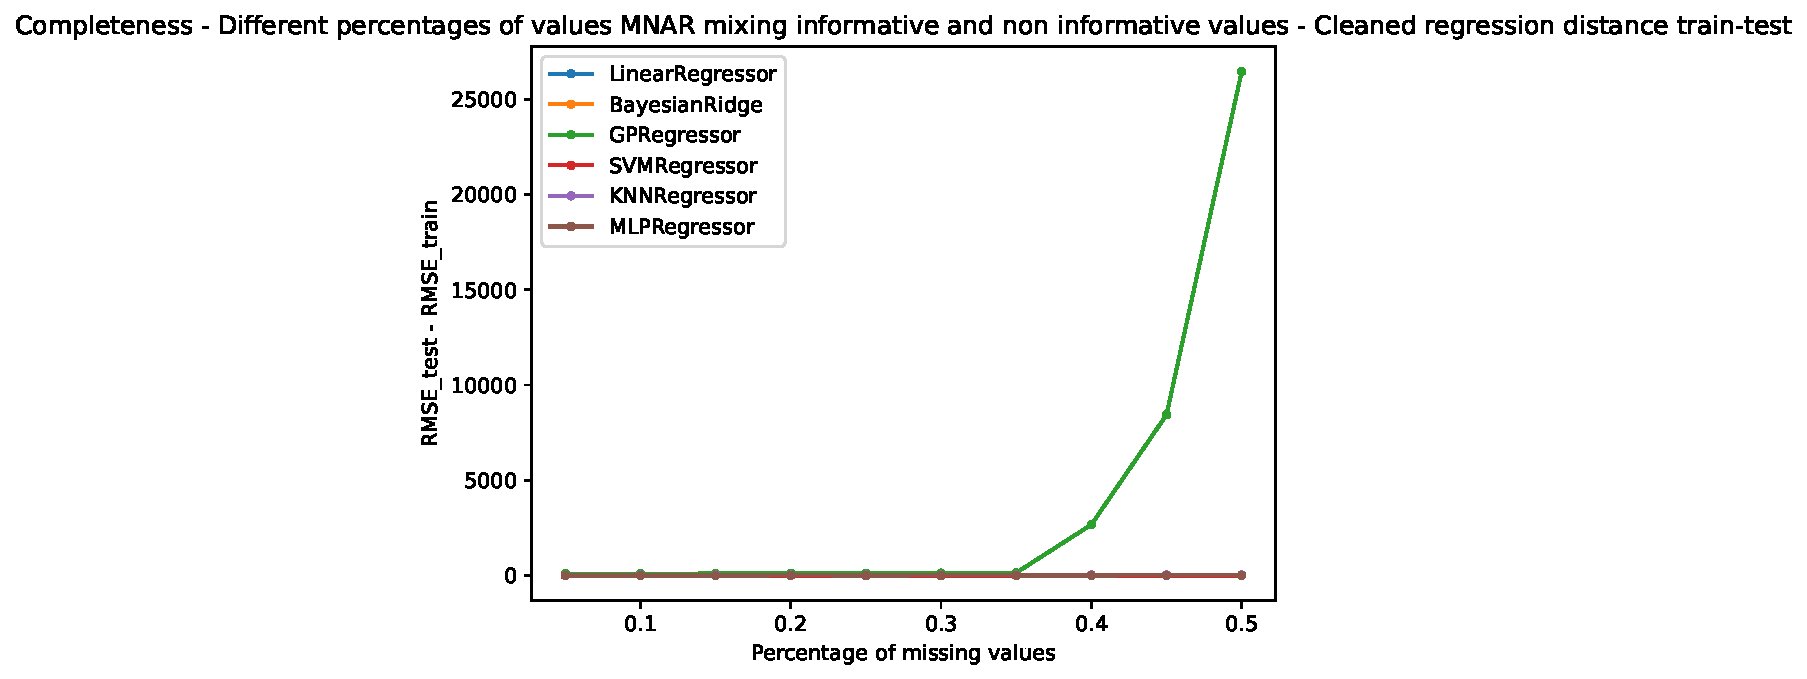
\includegraphics[scale=0.55]{Images/completeness/4.pdf}  
\end{figure}
\begin{figure}[H]
    \centering
    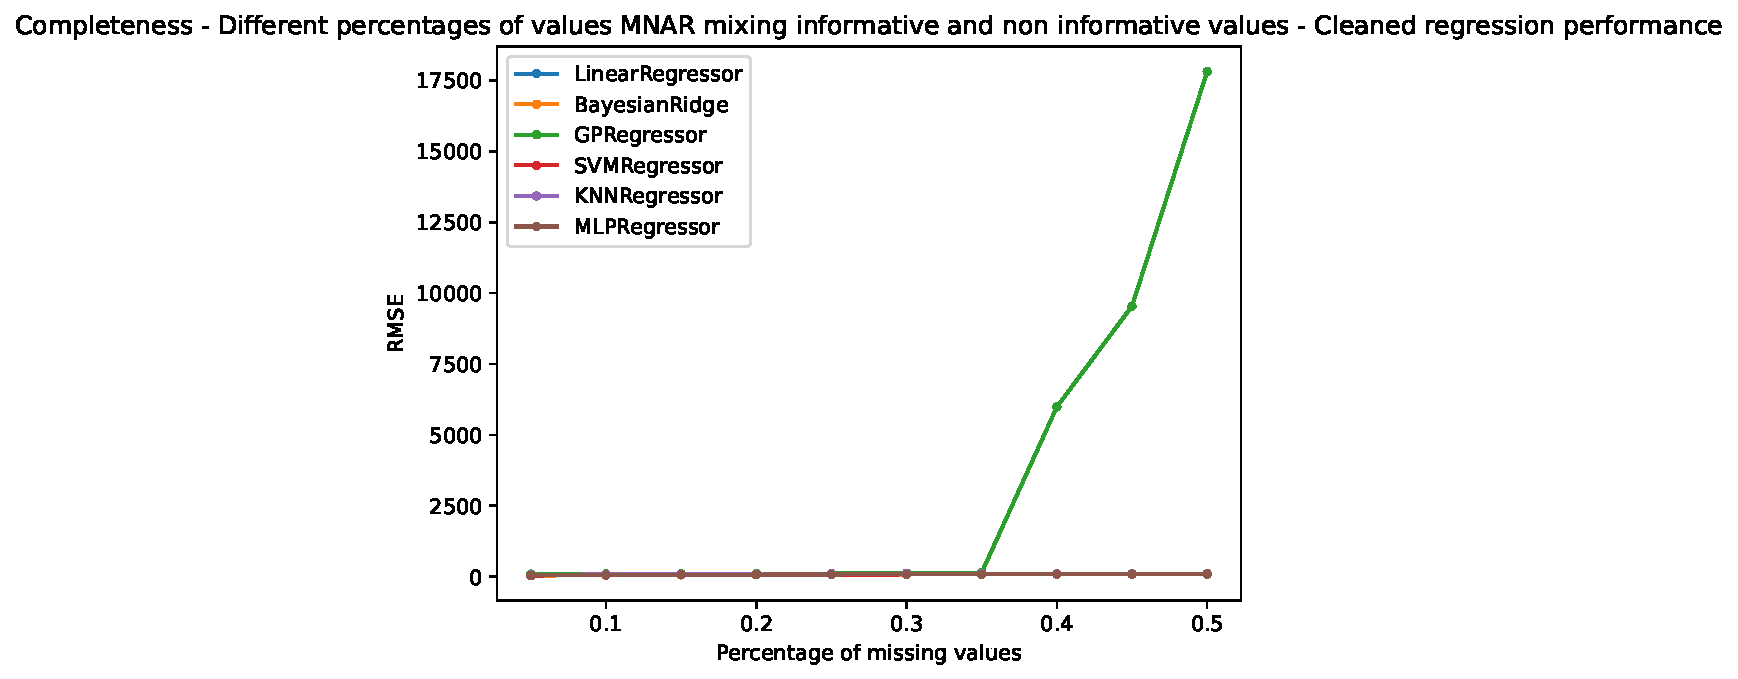
\includegraphics[scale=0.55]{Images/completeness/5.pdf}  
\end{figure}
\begin{figure}[H]
    \centering
    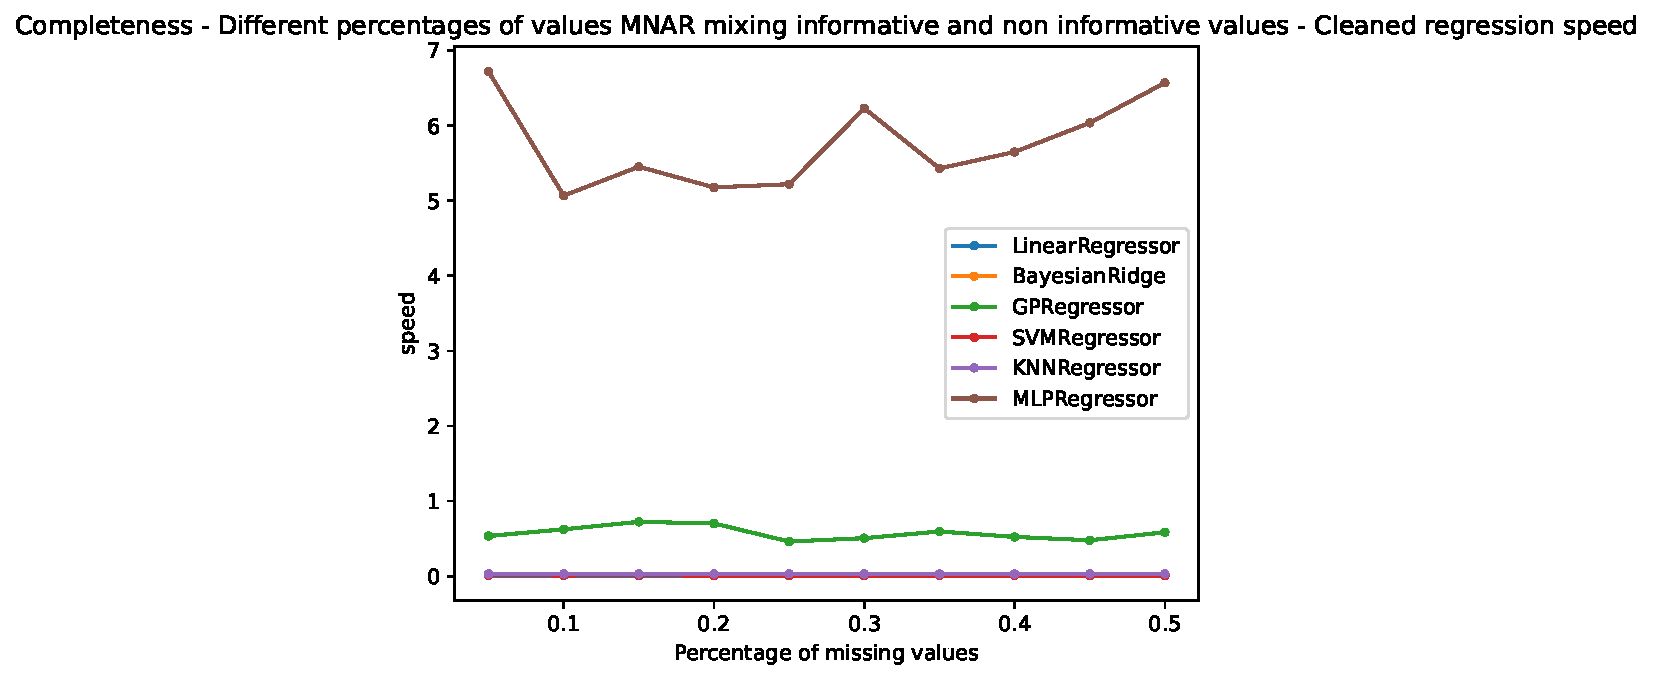
\includegraphics[scale=0.6]{Images/completeness/6.pdf}  
\end{figure}
\begin{figure}[H]
    \centering
    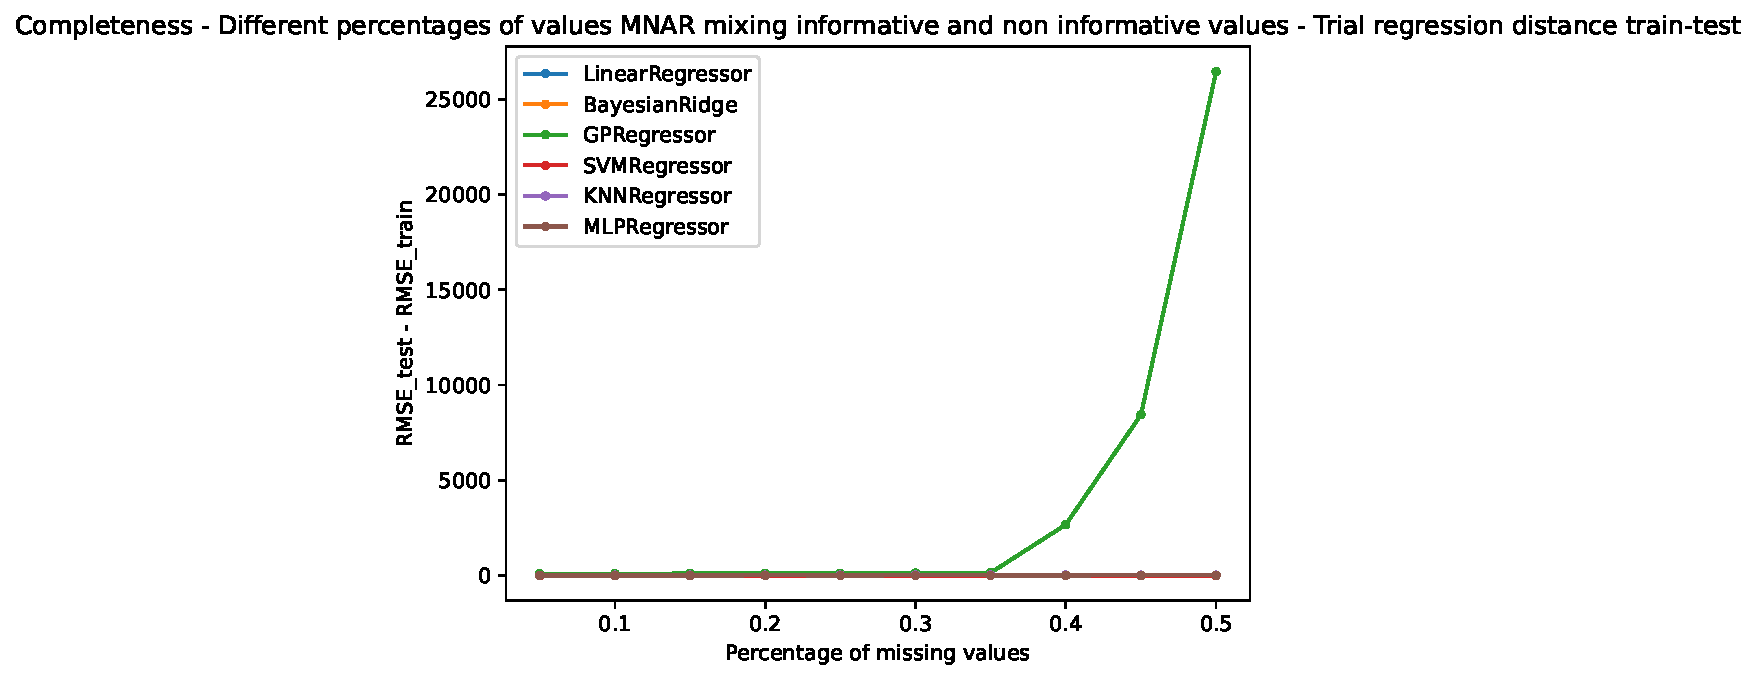
\includegraphics[scale=0.6]{Images/completeness/7.pdf}
\end{figure}
\begin{figure}[H]
    \centering
    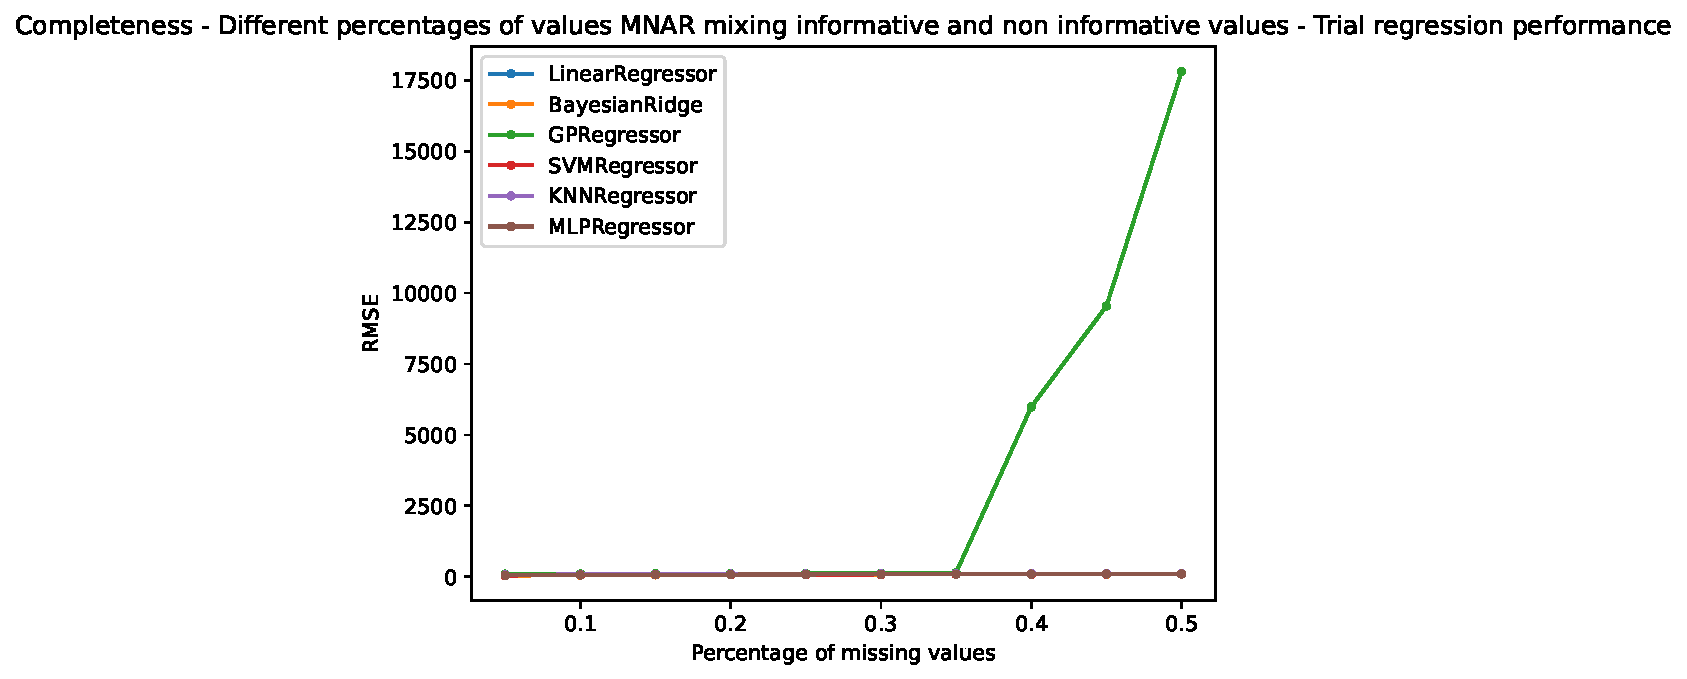
\includegraphics[scale=0.6]{Images/completeness/8.pdf}
\end{figure}
\begin{figure}[H]
    \centering
    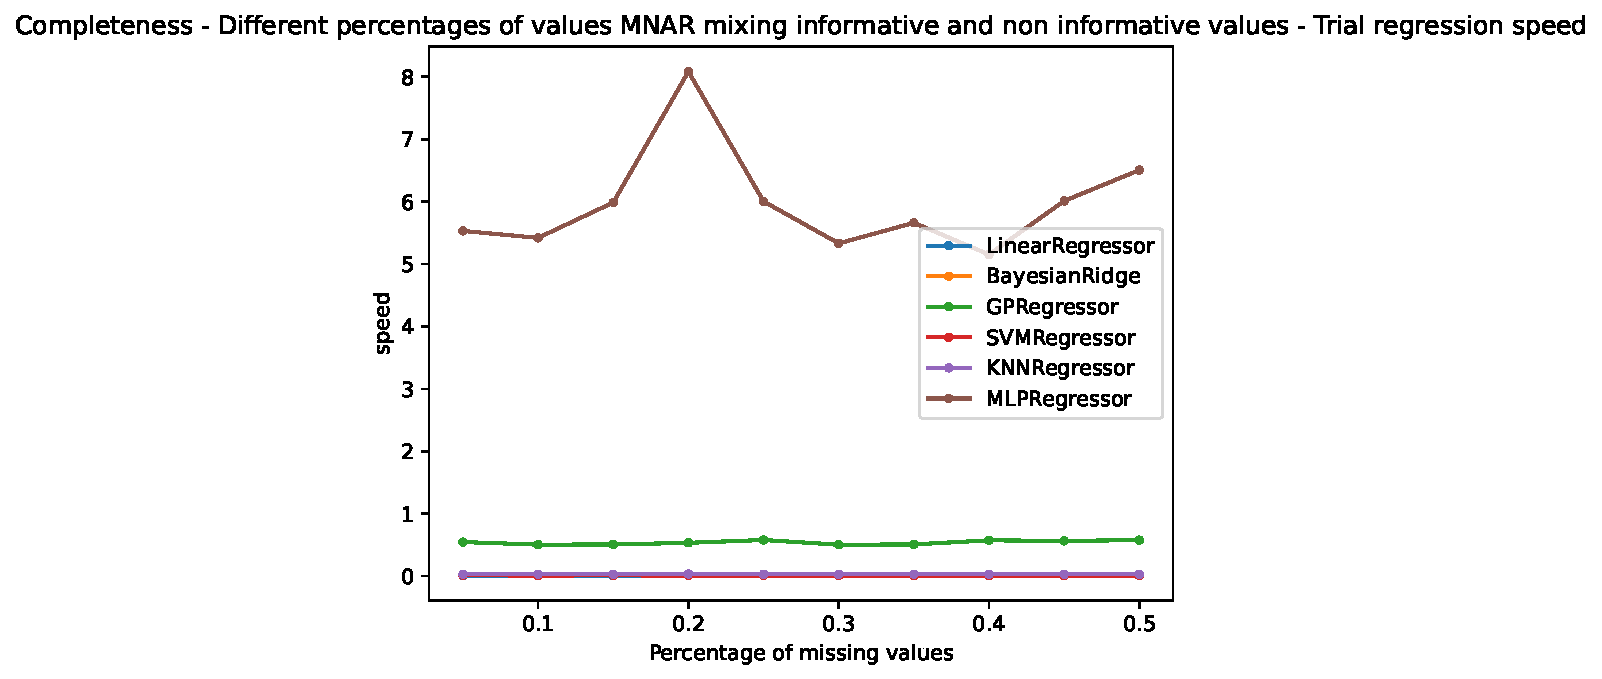
\includegraphics[scale=0.6]{Images/completeness/9.pdf}
\end{figure}
\begin{figure}[H]
    \centering
    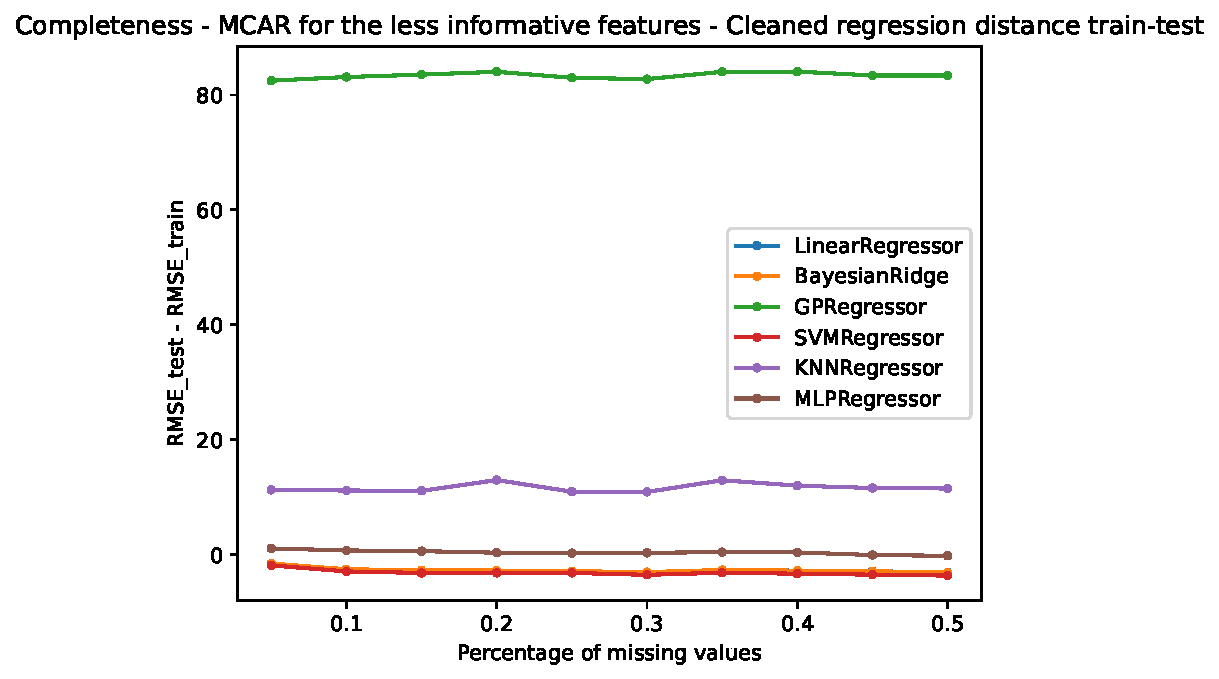
\includegraphics[scale=0.6]{Images/completeness/10.pdf}
\end{figure}
\begin{figure}[H]
    \centering
    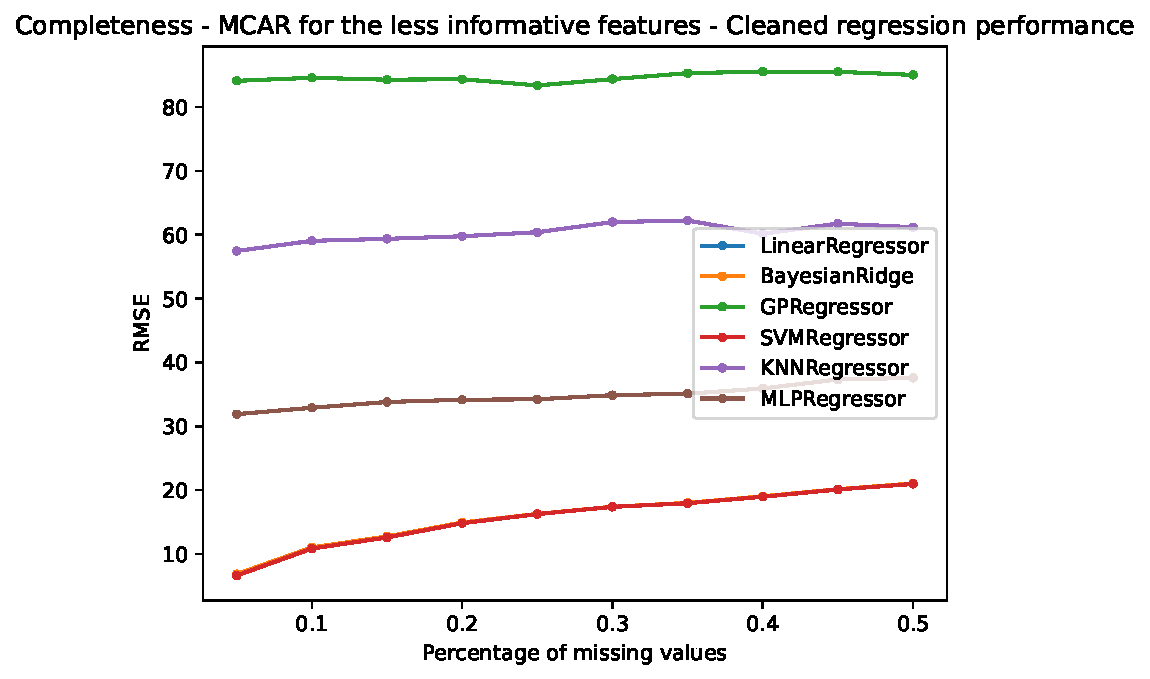
\includegraphics[scale=0.6]{Images/completeness/11.pdf}
\end{figure}
\begin{figure}[H]
    \centering
    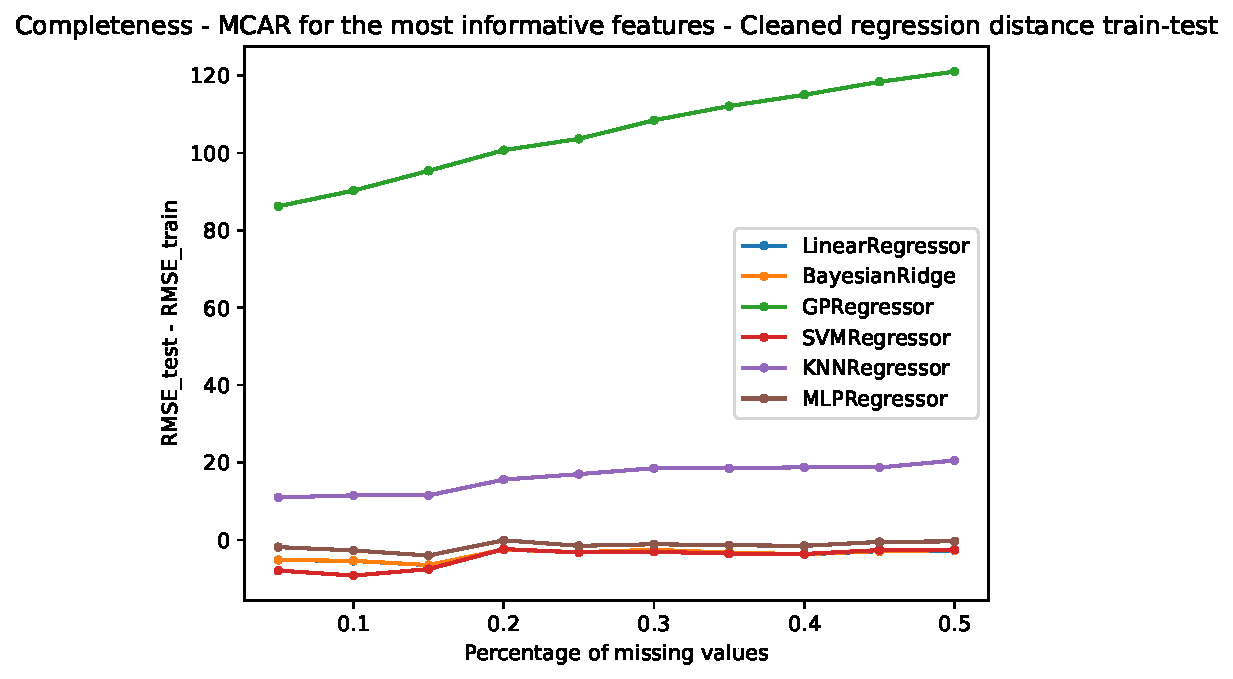
\includegraphics[scale=0.6]{Images/completeness/12.pdf}
\end{figure}
\begin{figure}[H]
    \centering
    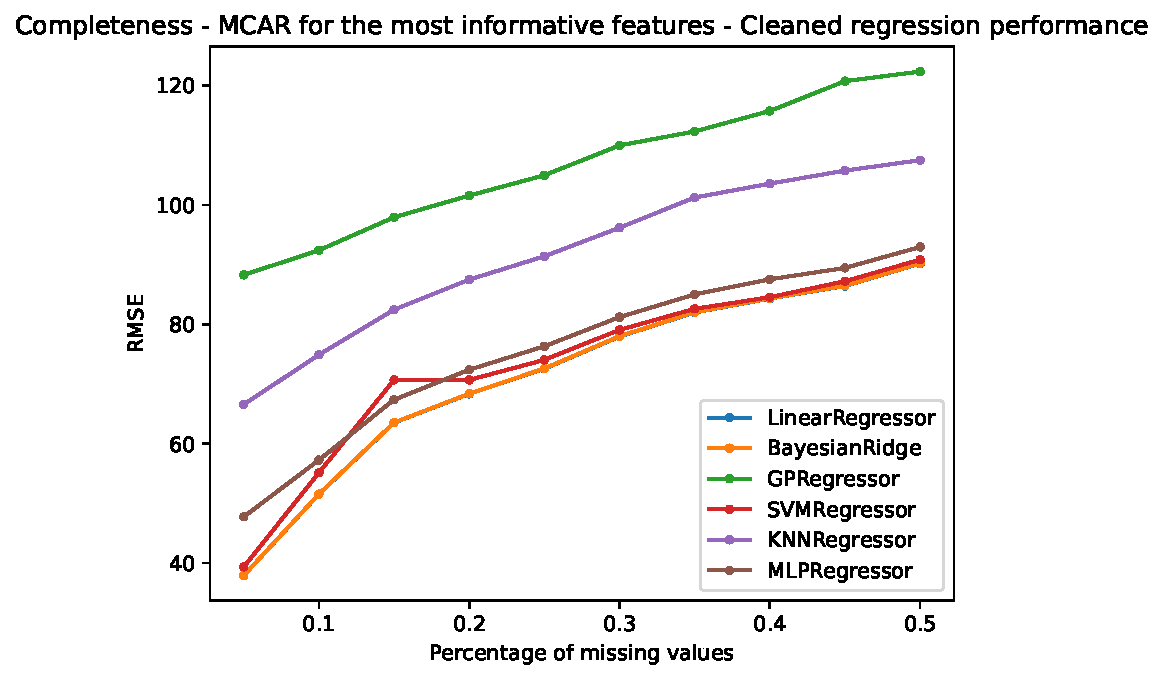
\includegraphics[scale=0.6]{Images/completeness/13.pdf}
\end{figure}
\begin{figure}[H]
    \centering
    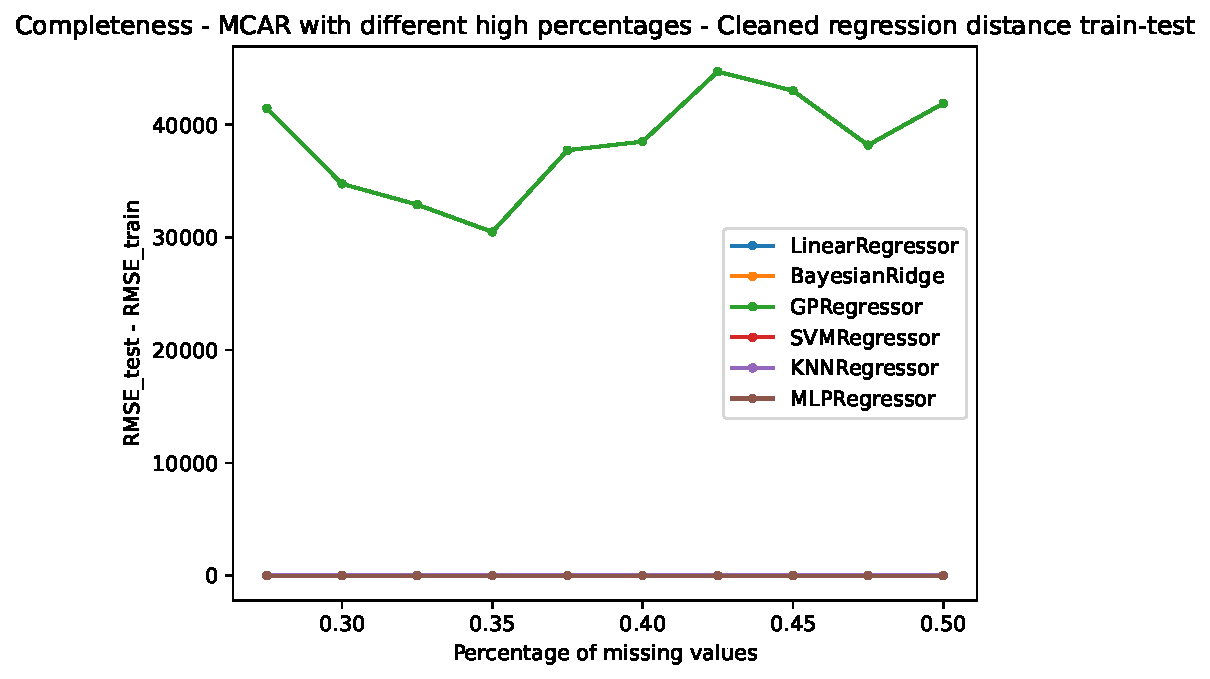
\includegraphics[scale=0.6]{Images/completeness/14.pdf}    
\end{figure}
\begin{figure}[H]
    \centering
    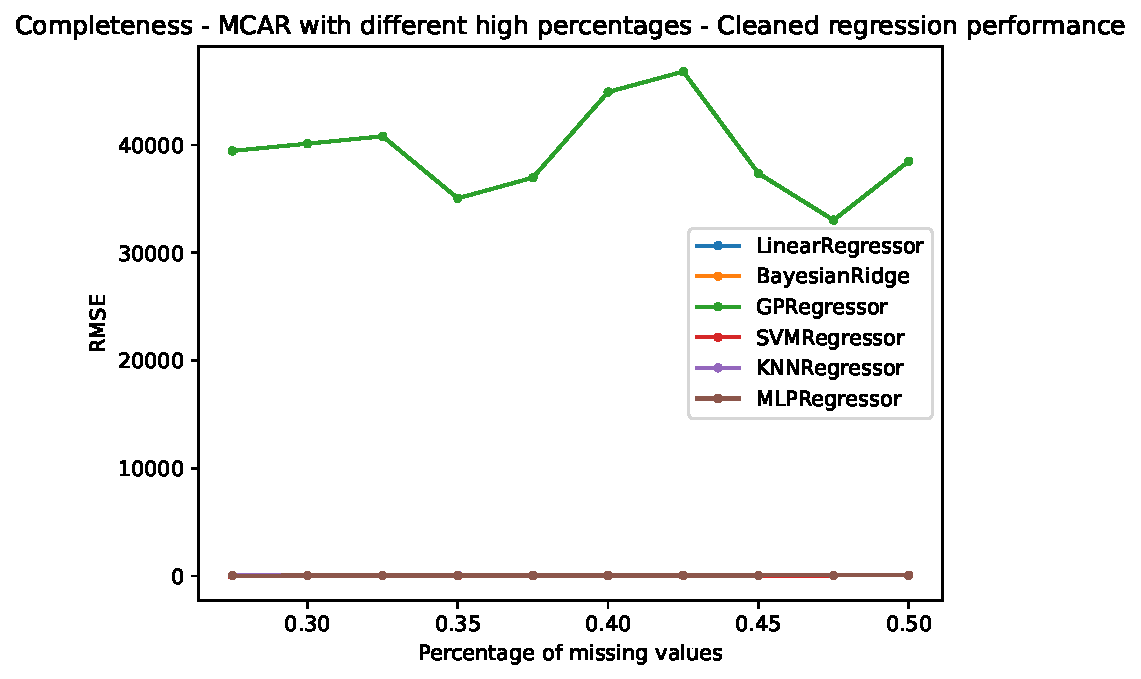
\includegraphics[scale=0.6]{Images/completeness/15.pdf}     
\end{figure}
\begin{figure}[H]
    \centering
    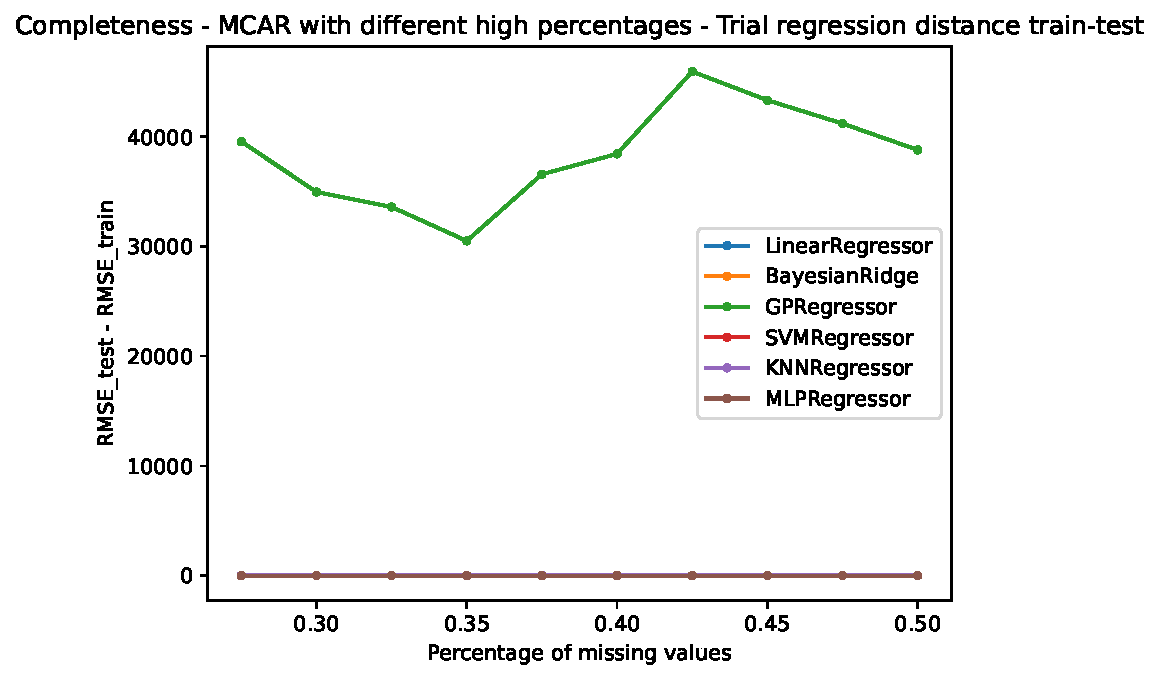
\includegraphics[scale=0.6]{Images/completeness/16.pdf}   
\end{figure}
\begin{figure}[H]
    \centering
    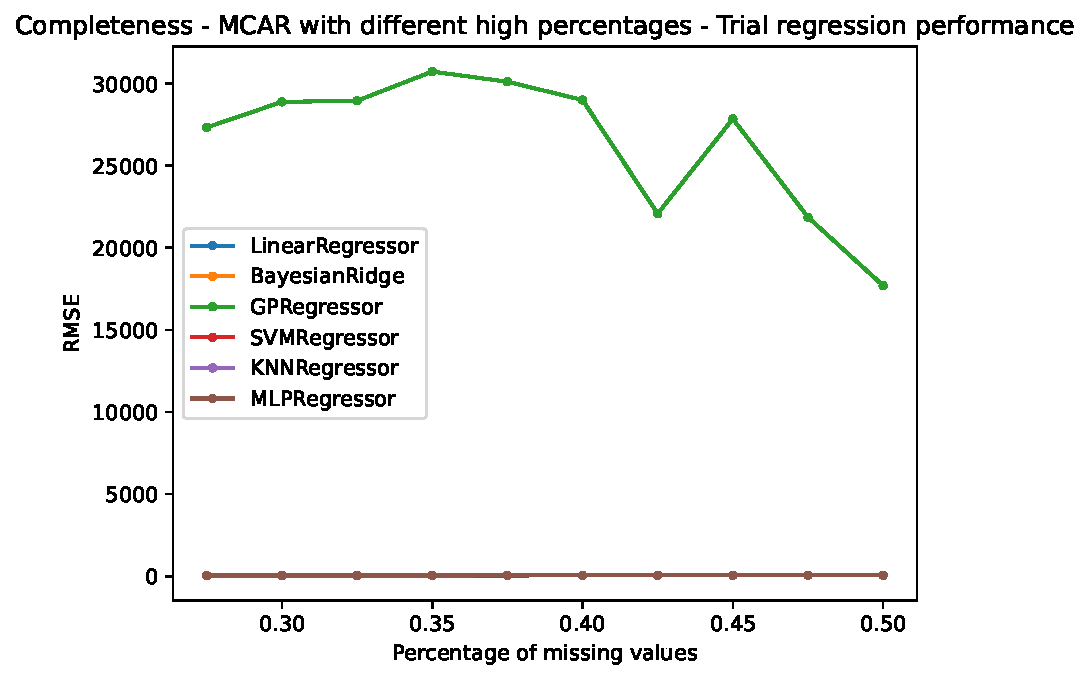
\includegraphics[scale=0.6]{Images/completeness/17.pdf}
\end{figure}


\newpage
\newpage
\section{Distinctness}
\label{sec:section_4_2}%

\subsection{Main results of the distinctness experiments}
\label{subsec:section_4_2_1}%

Based on the experiments conducted on the distinctness in a regression problem, we draw the following conclusions:
\begin{enumerate}
    \item Distinctness Impact on Model Performance:
        Model performance is notably affected by distinctness changes in the dataset. Generally, as distinctness percentages decrease, models tend to perform poorly. This is evident across various experiments involving different approaches to manipulating distinctness.
    \item GP Regressor's Sensitivity to Distinctness:
        The GP Regressor consistently exhibits poor performance under distinctness variations, struggling to construct a meaningful probability model based on altered targets. Its results are consistently worse than those of other models.
    \item Similarity in Train-Test Performance for Most Models:
        Across experiments, models, except GP Regressor and KNN Regressor, demonstrate similar performances on both training and testing sets. The distances between training and testing performances are generally close to zero, indicating a consistent generalization ability.
    \item Effect of Increased Distinctness Percentages:
        When distinctness percentages increase, resulting in lower percentages of distinct values, model performances tend to improve. However, performance eventually saturates to a single value as models lose a component of the search space, making it challenging to achieve high accuracy.
    \item Distinctness and Dataset Size Relationship:
        Distinctness of a single column significantly impacts the final model, as observed in experiments with fixed distinctness percentages and increasing dataset sizes. The fluctuating performance graph highlights the difficulty in determining the precise cause, emphasizing the need for careful consideration of distinctness in dataset design.
    \item Limited Influence of Algorithm Speed:
        The speed of the algorithms remains relatively stable across distinctness experiments. No remarkable changes in algorithm speed were observed, indicating that the computational efficiency of the models is not significantly influenced by variations in distinctness.
\end{enumerate}
To confirm our conclusions we show some of the most important graphs for distinctness.

\newpage
\begin{figure}
    \centering
    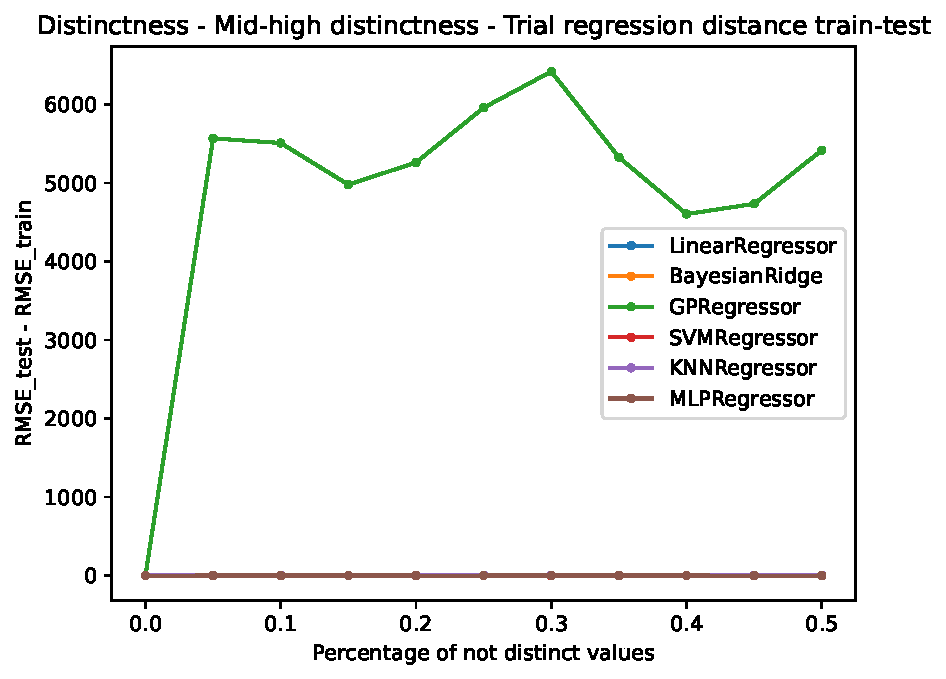
\includegraphics[scale=0.6]{Images/distinctness/dex1/Distinctness - Mid-high distinctness - Trial regression distance train-test.pdf}
\end{figure}
\begin{figure}
    \centering
    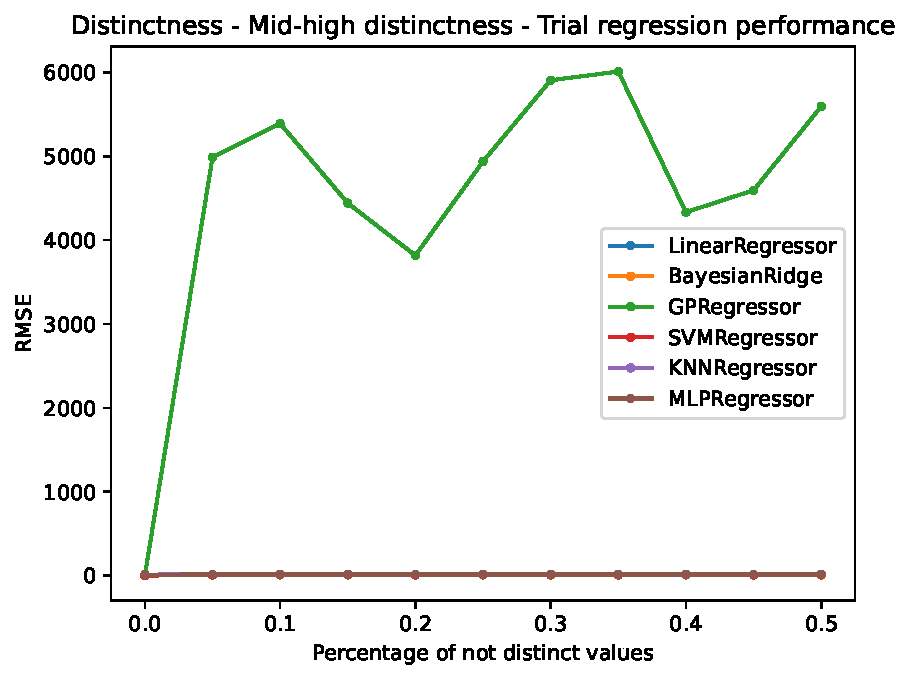
\includegraphics[scale=0.6]{Images/distinctness/dex1/Distinctness - Mid-high distinctness - Trial regression performance.pdf}
\end{figure}
\begin{figure}
    \centering
    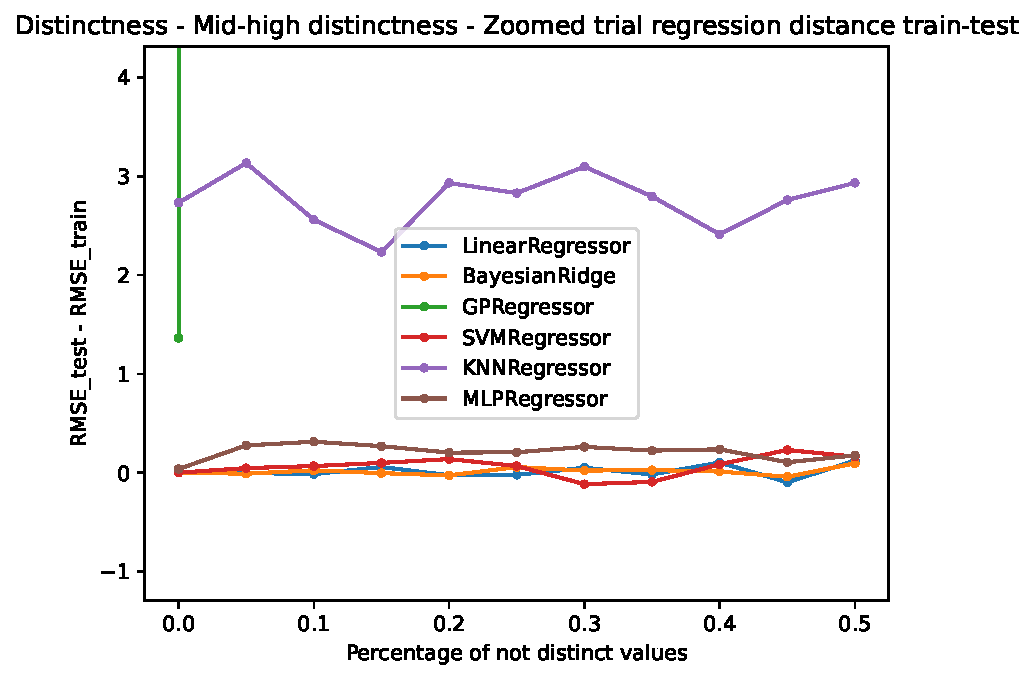
\includegraphics[scale=0.6]{Images/distinctness/dex1/Distinctness - Mid-high distinctness - Zoomed trial regression distance train-test.pdf}
\end{figure}
\begin{figure}
    \centering
    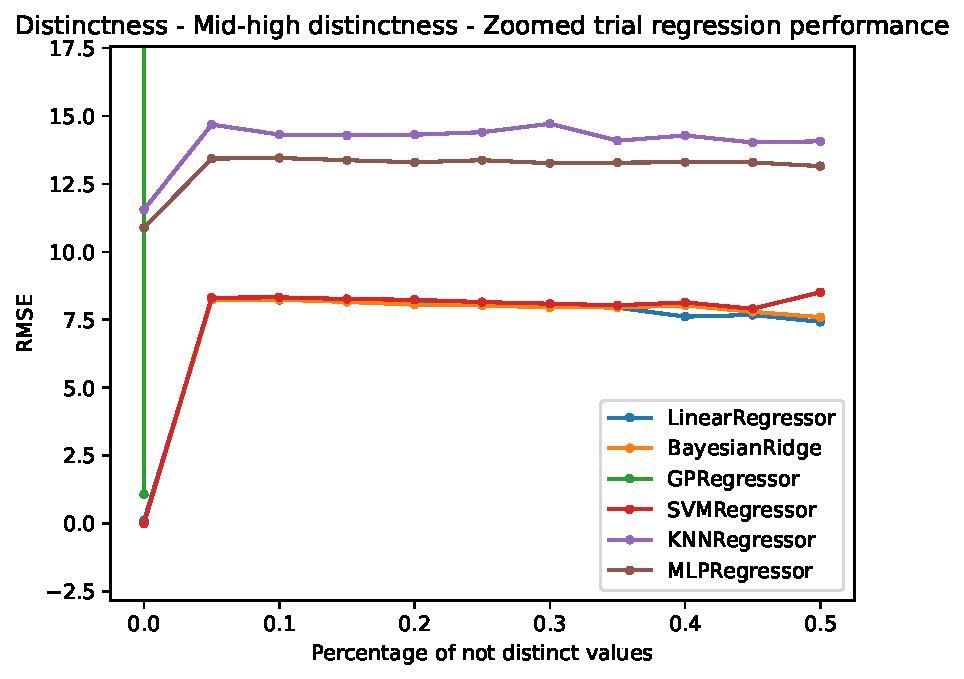
\includegraphics[scale=0.6]{Images/distinctness/dex1/Distinctness - Mid-high distinctness - Zoomed trial regression performance.pdf}
\end{figure}
\begin{figure}
    \centering
    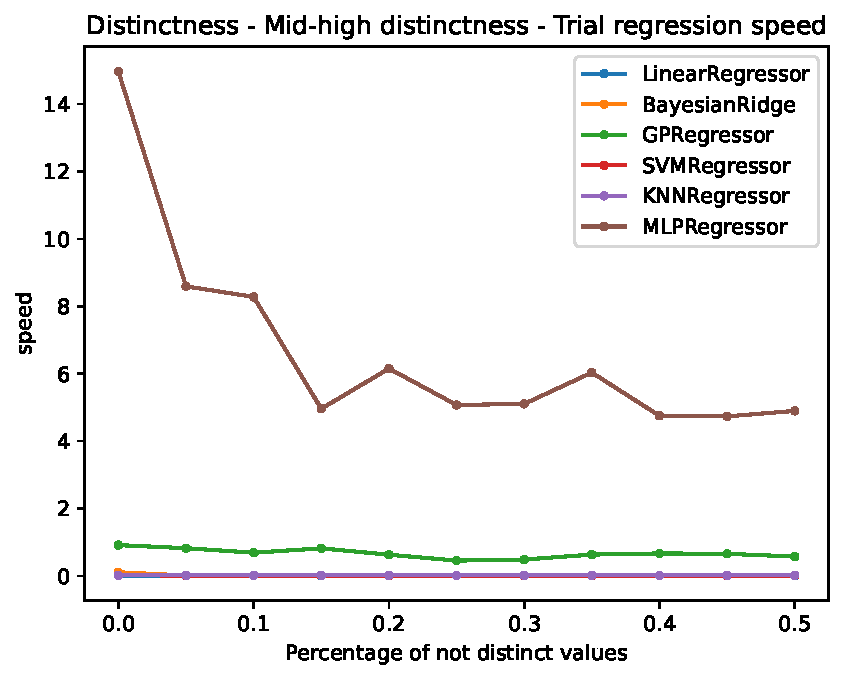
\includegraphics[scale=0.6]{Images/distinctness/dex1/Distinctness - Mid-high distinctness - Trial regression speed.pdf}
\end{figure}
\begin{figure}
    \centering
    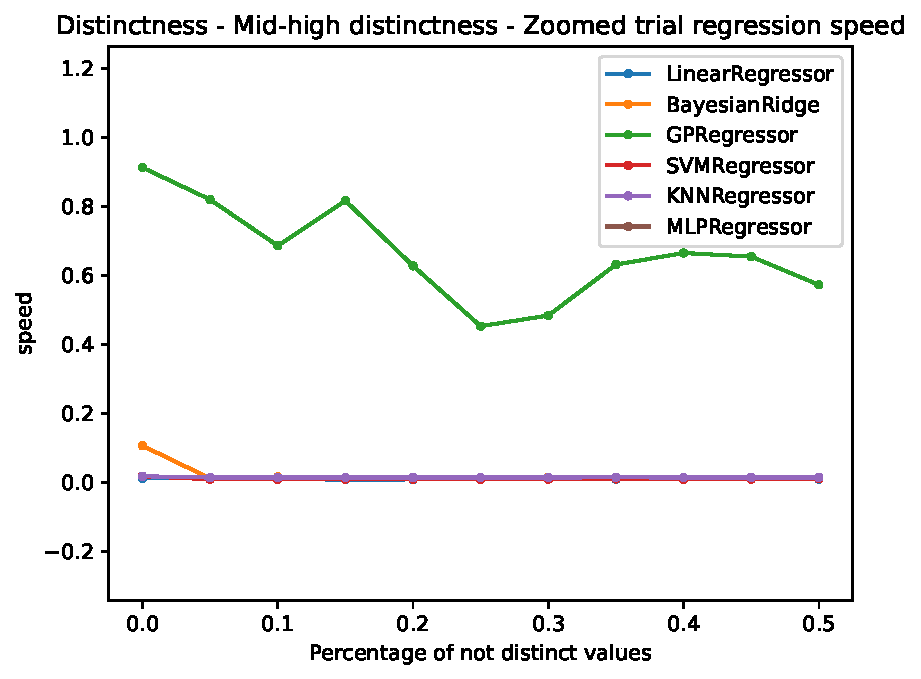
\includegraphics[scale=0.6]{Images/distinctness/dex1/Distinctness - Mid-high distinctness - Zoomed trial regression speed.pdf}
\end{figure}
    

    







\cleardoublepage
\begin{thebibliography}{100}
        \bibitem{github_reference} \textbf{GitHub repository that contains all the experiments mentioned in the document} \href{https://github.com/BiancaSavoiu/DIQ_project}{https://github.com/BiancaSavoiu/DIQproject}
    \end{thebibliography}
\end{document}
